% !TeX program = pdfLaTeX
\documentclass[12pt]{article}
\usepackage{amsmath}
\usepackage{graphicx,psfrag,epsf}
\usepackage{enumerate}
\usepackage{natbib}
\usepackage{textcomp}
\usepackage[hyphens]{url} % not crucial - just used below for the URL
\usepackage{hyperref}

%\pdfminorversion=4
% NOTE: To produce blinded version, replace "0" with "1" below.
\newcommand{\blind}{0}

% DON'T change margins - should be 1 inch all around.
\addtolength{\oddsidemargin}{-.5in}%
\addtolength{\evensidemargin}{-.5in}%
\addtolength{\textwidth}{1in}%
\addtolength{\textheight}{1.3in}%
\addtolength{\topmargin}{-.8in}%

%% load any required packages here



% tightlist command for lists without linebreak
\providecommand{\tightlist}{%
  \setlength{\itemsep}{0pt}\setlength{\parskip}{0pt}}

% From pandoc table feature
\usepackage{longtable,booktabs,array}
\usepackage{calc} % for calculating minipage widths
% Correct order of tables after \paragraph or \subparagraph
\usepackage{etoolbox}
\makeatletter
\patchcmd\longtable{\par}{\if@noskipsec\mbox{}\fi\par}{}{}
\makeatother
% Allow footnotes in longtable head/foot
\IfFileExists{footnotehyper.sty}{\usepackage{footnotehyper}}{\usepackage{footnote}}
\makesavenoteenv{longtable}



\begin{document}


\def\spacingset#1{\renewcommand{\baselinestretch}%
{#1}\small\normalsize} \spacingset{1}


%%%%%%%%%%%%%%%%%%%%%%%%%%%%%%%%%%%%%%%%%%%%%%%%%%%%%%%%%%%%%%%%%%%%%%%%%%%%%%

\if0\blind
{
  \title{\bf \emph{Pass-Through} Cambial: Uma análise para o Brasil}

  \author{
        Luca Klein \\
    Cedeplar, Universidade Federal de Minas Gerais\\
      }
  \maketitle
} \fi

\if1\blind
{
  \bigskip
  \bigskip
  \bigskip
  \begin{center}
    {\LARGE\bf \emph{Pass-Through} Cambial: Uma análise para o Brasil}
  \end{center}
  \medskip
} \fi

\bigskip
\begin{abstract}
O presente artigo se objetiva em analisar empiricamente a relação entre
o câmbio e o índice de preço brasileiro, o IPCA (Índice de Preços
Consumidor Amplo), no período de 2010 a 2022. Para tal, será feito um
prevê levantamento sobre a literatura e, posteriormente, a apresentasam
dos resultados empíricos obtidos através da metodologia de Vetor
Autoregressivo (VAR). No que tange a parte teórica, existem alguns tipos
de abordagem para o tema, tanto no âmbito microeconômico quanto no
macroeconômico. O trabalho, por sua vez, irá destacar somente a
abordagem macroeconômica no intuito de evidenciar a contaminação dos
preços domésticos pelo câmbio de uma maneira mais agregada. Pelo lado
dos resultados, a estimação revelou um baixo grau de repasse cambial
para os preços, uma vez que o período analisado apresenta vetores que
limitam esse tipo de dinâmica.
\end{abstract}

\noindent%
{\it Keywords:} Preços, Séries Temporais, Macroêconomia
\vfill

\newpage
\spacingset{1.45} % DON'T change the spacing!

\hypertarget{introduuxe7uxe3o}{%
\section{Introdução}\label{introduuxe7uxe3o}}

A ideia central do artigo é verificar como a variação na taxa de câmbio
afeta o índice de preço doméstico, tal fenômeno é mais conhecido na
literatura como o \emph{pass-through} do câmbio para nflação. Nesse
sentido, o grau de \emph{pass-through} da taxa de câmbio para a inflação
é definido como o impacto da taxa de câmbio nominal sobre os preços
domésticos, em que a evidência empírica relata um grau menor do que uma
unidade, de acordo com Campa \& Goldberg (2002). A motivação por trás do
trabalho vem da falta de estudos desse tipo para o caso brasiliero, ao
passo que não há uma convergência acerca do grau de \emph{pass-through}
nesses mesmos relatos.

Nos últimos anos, o Brasil se deparou com uma crise econômica em 2015 e
com a crise sanitária global, em que alguns efeitos foram a depreciação
da moeda nacional e a elevação do nível de preços. Pelo lado doméstico,
evidenciamos alguns descolamentos da inflação de sua meta, como no caso
de do ano de 2021. Pelo lado externo, ambas as crises resultaram em um
cenário de maior aversão ao riscos dos agentes frente ao Brasil, de tal
forma que pudemos verificar uma apreciação do dólar localmente.
Trabalhos como Goldberg \& Knetter (1997) e Campa \& Goldberg (2002)
demonstraram que os preços domésticos estão cada vez menos voláteis em
relação ao câmbio.

Do ponto de vista teórico, o assunto pode ser elaborado tanto pela
teoria microeconômica quanto pela macroeconômica, sendo essa última a
abordagem do artigo. Ademais, mesmo a perspectiva macroeconômica pode
ser dividida entre setores, contudo, o trabalho vai focar somente no que
tange a parte agregada. No que se refere a parte empírica, o artigo
elabora um VAR (Vetor Autoregressivo) para medir a contaminação do
câmbio nominal nos preços.

\hypertarget{literatura}{%
\section{Literatura}\label{literatura}}

Dentro da teoria, podemos referenciar algumas abordagens macroeconômicas
sobre o grau de \emph{pass-through.} De modo geral, existem vários
vetores de contaminação da inflação pelo câmbio, porém, tal dinâmica
fica mais evidente a partir do maior grau de abertura comercial, demanda
doméstica aquecida, participação das importações dentro da cesta de
consumo das famílias e firmas e, por fim, maiores desvios entre a taxa
de câmbio realizada frente a de equilíbrio. Em outras palavras, o
\emph{pass-through} é intensificado a partir do momento em que o consumo
doméstico apresenta alta dependência do comércio internacional, então
choques externos impactam com maior ênfase tais nações, seja pelo
reajuste dos preços relativos ou por questões relacionas a oferta e
demanda. Alguns trabalhos de cunho mais setorial conseguem testar de
maneira mais eficiente as afirmações acima, como no caso de Krugman \&
Obstfeld (1994) que alegam que os preços dos produtos não
comercializáveis devem ser definidos exclusivamente por fatores de
oferta e demanda domésticas, de modo que uma elevação dos preços dados
domesticamente favoreça uma redução no poder de compra da moeda corrente
do país.

A literatura empírica sobre o tema ganhou mais ênfase dentro da academia
a partir de 1980. Uma das vertentes mais levantadas no começo se baseava
em testar a Paridade do Poder de Compra (PPP) que alegava que deveria
existir um repasse completo da variação do câmbio para os preços. No
entanto, os resultados refutaram tal hipótese e chegaram à conclusão de
que o \emph{pass-through} não seria completo nem no curto prazo e nem no
longo prazo, de acordo com Maciel (2006). Em seus novos contornos, o
trabalho de Taylor (2000) traz levantamentos relevantes para o tema.
Segundo o autor, um contexto de regime de inflação baixa ou estável é
capaz de reduzir \emph{pass-through} mediante a redução do poder das
firmas no que se refere a formação de preços. Desta maneira, o fenômeno
deve ser determinado endogenamente em relação ao contexto inflacionário.
Em suma, Taylor (2000) alega que inflação reduzida e a política
monetária conduzem a um baixo \emph{pass-through} através do balizamento
das expectativas acerca das mudanças frequentes nos custos e preços.

Na mesma linha de Taylor (2000), Goldfajn \& Werlang (2000) sugerem que
o ambiente de baixa inflação dificulta os repasses. Nesse sentido, como
as variações de preços e custos são mais estáveis, as firmas tendem a
repassar menos os custos dados via câmbio. Ademais, Goldfajn \& Werlang
(2000) chegam à conclusão de que os principais determinantes para o
\emph{pass-through} são o hiato do produto, grau de abertura comercial e
taxa de câmbio real. Nesse sentido, há evidências de que quanto maior a
ociosidade da economia, maior a dificuldade de repasse cambial para os
preços. Isto é, diante de um cenário de expansão da economia, onde a
ociosidade dos fatores de produção é baixo, as firmas tendem a ter mais
facilidade para repassar os custos relacionados ao câmbio. No que tange
a taxa de câmbio real, estudos mencionam que tais taxas sobreapreciadas
colaboram para uma depreciação futura. Sendo assim, Goldfajn \& Werlang
(2000) reforçam tal perspectiva ao afirmar que a correções cambiais
mediante a depreciações em abundância implicariam em um ambiente de
aceleração inflacionária.

Outra contribuição importante veio de Romer (1993), principalmente pelo
lado da abertura comercial. Romer (1993) comenta que a abertura gera
efeitos sobre os determinantes da inflação no momento que o governo
exerce choque inesperado nos preços frente a uma desvalorização cambial.
Nessa linha, haveria um impacto sobre os benefícios de uma expansão do
produto em relação ao seu \emph{trade-off} com a inflação. Logo, segundo
o autor, o grau de abertura tem influência negativa sobre os incentivos
de produção doméstica e, portanto, corroborando a ideia de que o
\emph{pass-through} será maior quando esse cenário de demanda externa
prevalecer sobre a interna, à exceção de bens substitutos. Acerca do
\emph{trade-off} entre produto e inflação, Romer (1993) argumenta que um
maior grau de abertura comercial colabora com a alta da inflação no
momento de crescimento do produto o que, por sua vez, deve gerar uma
depreciação da taxa de câmbio e, consequentemente, alta nos preços
domésticos. O autor relata dois canais de transmissão dessa
contaminação. O primeiro se refere há um aumento acelerado dos custos do
câmbio para inflação via produtos importados. Enquanto o segundo, se dá
com a alta do nível geral de preços que impacta positivamente os bens
individuais, então com essa percepção e assumindo salários flexíveis, os
custos das firmas tenderiam a aumentar e, assim, também os reflexos
positivos sobre os preços dos bens domésticos. Em linhas gerais, um
cenário de crescimento do produto atrelado à uma economia com alto grau
de abertura comercial provoca uma expansão monetária e altas nos preços
domésticos.

\hypertarget{anuxe1lise-empuxedrica}{%
\section{Análise Empírica}\label{anuxe1lise-empuxedrica}}

\hypertarget{base-de-dados}{%
\subsection{Base de dados}\label{base-de-dados}}

\begin{enumerate}
\def\labelenumi{\arabic{enumi}.}
\item
  IPCA - Número-índice (base 1993 = 100) - divulgado pelo Instituto
  Brasileiro de Geografia e Estatística (IBGE)
\item
  Taxa de Câmbio (R\$/USD) - livre/venda - Média de período - divulgado
  pelo Banco Central
\item
  Petróleo Brent Futuros (R\$/USD) - divulgado pelo Fred St.~Louis
\item
  Produção Industrial Mensal(PIM) - Número índice com ajuste sazonal
  (base 2012=100) - divulgado pelo Instituto Brasileiro de Geografia e
  Estatística (IBGE)
\end{enumerate}

Os dados utilizados estão na periodicidade mensal e foi aplicada uma
função logarítmica sobre eles. Ademais, a estimação usufruiu de dados de
preços e atividade econômica, sendo que as variáveis PIM e petróleo são
\emph{proxys} de controle para estabelecer uma relação de demanda e
oferta, respectivamente, como sugerido em Alves \& Souza (2011). Por
fim, o período considerado é janeiro de 2010 a fevereiro de 2022 e todas
as variáveis foram tratadas como endógenas.

\hypertarget{teste-de-estacionariedade}{%
\subsection{Teste de Estacionariedade}\label{teste-de-estacionariedade}}

A partir do teste de Dickey-Fuller Aumentado (ADF) verificou-se que as
séries em nível aceitavam H0, ou seja, os dados são não estacionários.
Contudo, tomando a primeira diferença refutamos a hipótese nula, como
demostrado na tabela abaixo.

\hypertarget{tabela-1-teste-de-raiz-unituxe1ria}{%
\paragraph{Tabela 1: Teste de raiz
unitária}\label{tabela-1-teste-de-raiz-unituxe1ria}}

\begin{longtable}[]{@{}cccc@{}}
\toprule
Variável & Estatística & P-Valor & Status \\
\midrule
\endhead
IPCA & -1.6282 & 0.7313 & Nível \\
Câmbio & -2.9474 & 0.1819 & Nível \\
Petróleo & -1.4739 & 0.7955 & Nível \\
PIM & -2.8466 & 0.2239 & Nível \\
IPCA & -3.8991 & 0.01616 & Primeira Diferença \\
Câmbio & -3.7768 & 0.02214 & Primeira Diferença \\
Petróleo & -4.6761 & 0.01\textless{} & Primeira Diferença \\
PIM & -6.2335 & 0.01\textless{} & Primeira Diferença \\
\bottomrule
\end{longtable}

\hypertarget{seleuxe7uxe3o-de-defasagem}{%
\subsection{Seleção de Defasagem}\label{seleuxe7uxe3o-de-defasagem}}

Esta seção apresenta a seleção de defasagens a ser utilizada no modelo
VAR, com defasagem máxima de 12 meses à frente. Os critérios
considerados são:

\begin{enumerate}
\def\labelenumi{\arabic{enumi}.}
\item
  AIC: critério de informação de Akaike
\item
  HQ: critério de informação de Hannan-Quinn
\item
  SC: critério de informação de Schwarz
\item
  FPE: critério de previsão de erro final
\end{enumerate}

\hypertarget{tabela-2-estatuxedstica-dos-crituxe9rios}{%
\paragraph{Tabela 2: Estatística dos
Critérios}\label{tabela-2-estatuxedstica-dos-crituxe9rios}}

\begin{longtable}[]{@{}rrrrr@{}}
\toprule
Lag & AIC(n) & HQ(n) & SC(n) & FPE(n) \\
\midrule
\endhead
1 & -30.01287 & -29.83625 & -29.57823 & 0 \\
2 & -29.90253 & -29.58461 & -29.12018 & 0 \\
3 & -29.85442 & -29.39521 & -28.72436 & 0 \\
4 & -29.94904 & -29.34853 & -28.47127 & 0 \\
5 & -29.84363 & -29.10182 & -28.01814 & 0 \\
6 & -29.73242 & -28.84932 & -27.55923 & 0 \\
7 & -29.74114 & -28.71674 & -27.22024 & 0 \\
8 & -29.70645 & -28.54075 & -26.83783 & 0 \\
9 & -29.63678 & -28.32979 & -26.42045 & 0 \\
10 & -29.48321 & -28.03492 & -25.91917 & 0 \\
11 & -29.35174 & -27.76215 & -25.43999 & 0 \\
12 & -29.34115 & -27.61027 & -25.08169 & 0 \\
\bottomrule
\end{longtable}

Por unanimidade, os critérios sugerem que a defasagem dentro do modelo
deve ser de 1 período, como evidenciado a seguir

\hypertarget{tabela-3-defasagens}{%
\paragraph{Tabela 3: Defasagens}\label{tabela-3-defasagens}}

\begin{longtable}[]{@{}rrrr@{}}
\toprule
AIC(n) & HQ(n) & SC(n) & FPE(n) \\
\midrule
\endhead
1 & 1 & 1 & 1 \\
\bottomrule
\end{longtable}

\hypertarget{teste-de-quebra-estrutural}{%
\subsection{Teste de Quebra
Estrutural}\label{teste-de-quebra-estrutural}}

O intuito por trás desse teste é verificar se existe alguma quebra
estrutural nas séries, desta maneira entender se há alguma diferença
significativa entre os parâmetros estimados que estabelecem a relação
entre as variáveis. Para tal, o artigo utilizou a método de CUSUM que se
baseia na soma acumulada dos resíduos recursivos e detecta a
instabilidade da variável quando os dados ultrapassam a área delimitada
por duas linhas críticas de 5\% de significância. Ao final do teste
verificou-se que não há quebras estruturais nas séries.

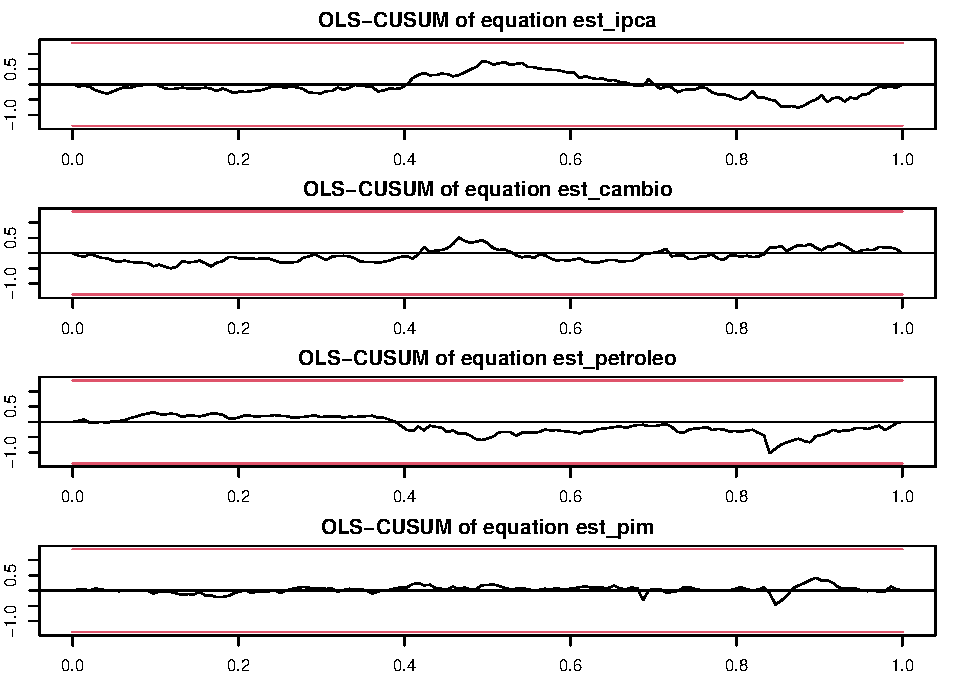
\includegraphics{artigo_files/figure-latex/unnamed-chunk-4-1.pdf}

\hypertarget{modelo}{%
\subsection{Modelo}\label{modelo}}

O sistema de equações gerados a partir da metodologia comentada e dos
critérios elencados acima gerou os seguintes parâmetros:

\hypertarget{tabela-4.1-ipca}{%
\paragraph{Tabela 4.1: IPCA}\label{tabela-4.1-ipca}}

\begin{longtable}[]{@{}rrrrr@{}}
\toprule
est\_ipca.l1 & est\_cambio.l1 & est\_petroleo.l1 & est\_pim.l1 &
const \\
\midrule
\endhead
0.5892862 & 0.0081637 & 0.0068322 & -0.0048094 & 0.0019451 \\
\bottomrule
\end{longtable}

\hypertarget{tabela-4.2-taxa-de-cuxe2mbio}{%
\paragraph{Tabela 4.2: Taxa de
Câmbio}\label{tabela-4.2-taxa-de-cuxe2mbio}}

\begin{longtable}[]{@{}rrrrr@{}}
\toprule
est\_ipca.l1 & est\_cambio.l1 & est\_petroleo.l1 & est\_pim.l1 &
const \\
\midrule
\endhead
0.0186154 & 0.1815868 & -0.066272 & -0.1025657 & 0.0056735 \\
\bottomrule
\end{longtable}

\hypertarget{tabela-4.3-petruxf3leo}{%
\paragraph{Tabela 4.3: Petróleo}\label{tabela-4.3-petruxf3leo}}

\begin{longtable}[]{@{}rrrrr@{}}
\toprule
est\_ipca.l1 & est\_cambio.l1 & est\_petroleo.l1 & est\_pim.l1 &
const \\
\midrule
\endhead
-1.475793 & 0.160552 & 0.2038139 & -0.5266126 & 0.0068239 \\
\bottomrule
\end{longtable}

\hypertarget{tabela-4.4-pim}{%
\paragraph{Tabela 4.4: PIM}\label{tabela-4.4-pim}}

\begin{longtable}[]{@{}rrrrr@{}}
\toprule
est\_ipca.l1 & est\_cambio.l1 & est\_petroleo.l1 & est\_pim.l1 &
const \\
\midrule
\endhead
-0.6239632 & -0.0210411 & 0.138887 & -0.097003 & 0.0017495 \\
\bottomrule
\end{longtable}

Por se tratar de modelos log-log, podemos interpretar os parâmetros como
elasticidades. Então, por exemplo, no caso do IPCA uma variação de 1\%
no câmbio defasado em 1 período está associado a uma variação, em média,
de 0,0081\% no IPCA no período de referência.

\hypertarget{correlauxe7uxe3o-serial}{%
\subsection{Correlação Serial}\label{correlauxe7uxe3o-serial}}

Para testar se os resíduos são independentes e não carregam nenhuma
informação relevante para o modelo utiliza-se o Teste de Portmanteau, em
que a hipótese nula do teste é de que os resíduos são
autocorrelacionados.

\hypertarget{tabela-5-teste-de-portmanteau}{%
\paragraph{Tabela 5: Teste de
Portmanteau}\label{tabela-5-teste-de-portmanteau}}

\begin{longtable}[]{@{}cl@{}}
\toprule
Chi - Quadrado & P-valor \\
\midrule
\endhead
198,94 & 0,1135 \\
\bottomrule
\end{longtable}

Como o P-valor \textgreater{} 0,05, podemos rejeitar H0 e concluir que
não há autocorrelação serial no modelo

\hypertarget{heterocedasticidade}{%
\subsection{Heterocedasticidade}\label{heterocedasticidade}}

Para testar se os resíduos apresentam variância constante, tomamos o
Teste ARCH multivariado que assume H0 como a presença de
heterocedasticidade.

\hypertarget{tabela-6-teste-arch}{%
\paragraph{Tabela 6: Teste ARCH}\label{tabela-6-teste-arch}}

\begin{longtable}[]{@{}cc@{}}
\toprule
Chi - Quadrado & P-valor \\
\midrule
\endhead
1258,8 & 0,1162 \\
\bottomrule
\end{longtable}

Como o P-valor \textgreater{} 0,05, podemos rejeitar H0 e concluir que
os resíduos são homocedásticos.

\hypertarget{causalidade}{%
\subsection{Causalidade}\label{causalidade}}

Dentro do universo dos modelos VAR a correlação, em grande medida, não é
a maneira mais adequada de se infererir relações entre as séries. Nesse
sentido, traçar causalidade entre as variáveis pode levantar maiores
evidências de relações entre elas. Portanto, aplicou-se o Teste de
Causalidade de Granger, em que nossa hipótese nula se baseia na ausência
de causalidade. Primeiramente, cabe avaliar se há causalidade de maneira
agregada, sendo que os resultados são apresentados na tabela 7. Em
segundo lugar, cabe traçar a causalidade individualmente entre as
variáveis, cujos resultados estão expostos na tabela 8.

\hypertarget{tabela-7-teste-de-granger}{%
\paragraph{Tabela 7: Teste de Granger}\label{tabela-7-teste-de-granger}}

\begin{longtable}[]{@{}ccc@{}}
\toprule
Variável & Teste-F & P-Valor \\
\midrule
\endhead
IPCA & 0.40008 & 0.753 \\
Câmbio & 0.61943 & 0.6026 \\
Petróleo & 18.46 & 0.01\textless{} \\
PIM & 2.0794 & 0.1019 \\
\bottomrule
\end{longtable}

Via tabela 7, a um nível de significância de 5\%, verificou-se que
somente há causalidade no sentido de Granger para a série de Petróleo,
nas demais aceitamos a hipótese nula.

\hypertarget{tabela-8-teste-de-granger}{%
\paragraph{Tabela 8: Teste de Granger}\label{tabela-8-teste-de-granger}}

\begin{longtable}[]{@{}ccc@{}}
\toprule
Variável & Teste-F & P-Valor \\
\midrule
\endhead
IPCA vs Câmbio & 0.07126336 & 0.7898962 \\
Câmbio vs IPCA & 0.0096 & 0.922 \\
IPCA vs Petróleo & 7.836 & 0.00584 \\
Petróleo vs IPCA & 0.4775 & 0.4907 \\
IPCA vs PIM & 0.0862 & 0.7695 \\
PIM vs IPCA & 0.3737 & 0.542 \\
Câmbio vs Petróleo & 6.3853 & 0.01261 \\
Petróleo vs Câmbio & 0.8044 & 0.3713 \\
Câmbio vs PIM & 1.6994 & 0.1945 \\
PIM vs Câmbio & 4.8334 & 0.02954 \\
Petróleo vs PIM & 1.1879 & 0.308 \\
PIM vs Petróleo & 50.36 & 0.01\textless{} \\
\bottomrule
\end{longtable}

A partir da tabela, a interpretação é de que a variável da esquerda
causa a da direita no sentido de Granger. Logo, com 95\% de confiança,
há evidências de que uma variação no IPCA causa Petróleo, assim como o
câmbio. Na sequência, existem evidências de que câmbio causa petróleo.
No que se refere à PIM, a variável de demanda, verificou-se que ela
causa câmbio, algo esperado, tendo em vista que a demanda tem
influências sobre o comportamento da variável, segundo a teoria exposta.
Outra relação espera é PIM causando Petróleo, isto é, demanda causando
oferta.

Ademais, vale destacar a falta de causalidade entre câmbio e IPCA, sendo
assim, podemos elencar alguns motivos que vem em linha com Taylor (2000)
e Goldfajn \& Werlang (2000). O primeiro deles é de que o período
analisado é composto por uma inflação controlada na maioria dos anos.
Mesmo com a mudança do intervalo da banda de 2 p.p. para 1.5 p.p em
2017, à exceção de 2015 e 2021 que o inflação supera a banda
estabelecida, os demais anos o IPCA se encontra dentro dos intervalos,
ou seja, estável. Um segundo condicionante para tal, diz respeito aos
anos de baixo crescimento e alta capacidade ociosa o que, por sua vez,
favorece a causalidade nula entre as séries em destaque.

\hypertarget{tabela-9-meta-e-ipca-realizado}{%
\paragraph{Tabela 9: Meta e IPCA
Realizado}\label{tabela-9-meta-e-ipca-realizado}}

\begin{longtable}[]{@{}
  >{\centering\arraybackslash}p{(\columnwidth - 8\tabcolsep) * \real{0.0822}}
  >{\centering\arraybackslash}p{(\columnwidth - 8\tabcolsep) * \real{0.1370}}
  >{\centering\arraybackslash}p{(\columnwidth - 8\tabcolsep) * \real{0.2055}}
  >{\centering\arraybackslash}p{(\columnwidth - 8\tabcolsep) * \real{0.2877}}
  >{\centering\arraybackslash}p{(\columnwidth - 8\tabcolsep) * \real{0.2877}}@{}}
\toprule
\begin{minipage}[b]{\linewidth}\centering
Ano
\end{minipage} & \begin{minipage}[b]{\linewidth}\centering
Meta (\%)
\end{minipage} & \begin{minipage}[b]{\linewidth}\centering
Realizado (\%)
\end{minipage} & \begin{minipage}[b]{\linewidth}\centering
Limite Superior (\%)
\end{minipage} & \begin{minipage}[b]{\linewidth}\centering
Limite Inferior (\%)
\end{minipage} \\
\midrule
\endhead
2012 & 4.5 & 5.8 & 6.5 & 2.5 \\
2013 & 4.5 & 5.9 & 6.5 & 2.5 \\
2014 & 4.5 & 6.4 & 6.5 & 2.5 \\
2015 & 4.5 & 10.7 & 6.5 & 2.5 \\
2016 & 4.5 & 6.3 & 6.5 & 2.5 \\
2017 & 4.5 & 3.0 & 6.0 & 3.0 \\
2018 & 4.5 & 3.8 & 6.0 & 3.0 \\
2019 & 4.25 & 4.3 & 5.75 & 2.75 \\
2020 & 4.0 & 4.5 & 5.5 & 2.5 \\
2021 & 3.75 & 10.1 & 5.25 & 2.25 \\
\bottomrule
\end{longtable}

Fonte: Banco Central do Brasil

\hypertarget{funuxe7uxe3o-impulso-resposta}{%
\subsection{Função Impulso
Resposta}\label{funuxe7uxe3o-impulso-resposta}}

A estimação de funções impulso resposta, assim como os testes de
causalidade, são capazes de trazer evidências mais interresantes para
relação entre as variáveis do que a correlação. Então, a ideia por trás
do procedimento é bem intuitiva, dar um choque em alguma variável e
observar o comportamento de outra variável até o choque se dissipar,
tendo em vista que modelos estáveis apresentam um comportamento de de
convergência das variáveis para sua tedência no longo prazo. No caso do
VAR estimado para o artigo, os resultados apontam que existe
estabilidade como demonstado pelo teste de CUSUM e pelas raízes
unitárias dentro do círculo unitário. Desta maneira, o artigo usufruiu
da função impulso resposta com choque de 12 períodos a frente. Os
gráficos que esboçam os resultados consideram a variável de resposta no
eixo Y e estão no anexo.

No que tange aos resultados, a função trouxe um impacto positivo para o
IPCA dado o choque em câmbio. Quando invertemos o choque, observou-se,
em um primeiro momento, um reflexo negativo no câmbio, contudo, a
relação se inverte à medida que os períodos avançam. Pelo lado da
oferta, um impulso resposta no IPCA evidenciou um comportamento positivo
sobre os preços, ao mesmo tempo que a dinâmica do impulso no IPCA frente
a oferta demonstrou uma variação positiva e gradualmente a inversão do
impacto para o campo negativo. A demanda, por sua vez, acusou reflexos
negativos sobre os preços, enquanto o choque do IPCA para demanda
demonstrou um efeito ligeiramente positivo nos primeiros períodos até o
ponto que a dinâmica se inverte. Em outras palavras, um choque positivo
de preço gera influências negativas para atividade econômica à medida
que o tempo avança, tal comportamento também é evidenciado por impulsos
via câmbio.

\hypertarget{decomposiuxe7uxe3o-de-variuxe2ncia}{%
\subsection{Decomposição de
Variância}\label{decomposiuxe7uxe3o-de-variuxe2ncia}}

A decomposição da variância do erro de previsão é baseada nas matrizes
de coeficiente de impulso resposta ortogonalizadas que permitem analisar
a contribuição de uma variável para previsão de outra série. Nesse
sentido, uma das métricas para o cálculo do \emph{pass-through} é a
partir da decomposição da variância o IPCA, segundo Bueno (2011). A
tabela 10 demonstra os resultados a partir de um choque de 12 períodos a
frente.

\hypertarget{tabela-10.1-ipca}{%
\paragraph{Tabela 10.1: IPCA}\label{tabela-10.1-ipca}}

\begin{longtable}[]{@{}rrrr@{}}
\toprule
est\_ipca & est\_cambio & est\_petroleo & est\_pim \\
\midrule
\endhead
1.0000000 & 0.0000000 & 0.0000000 & 0.0000000 \\
0.9528685 & 0.0000344 & 0.0456231 & 0.0014740 \\
0.9384389 & 0.0010248 & 0.0565263 & 0.0040100 \\
0.9358104 & 0.0020442 & 0.0573690 & 0.0047764 \\
0.9352163 & 0.0024499 & 0.0573809 & 0.0049529 \\
0.9350268 & 0.0025745 & 0.0573945 & 0.0050042 \\
0.9349566 & 0.0026142 & 0.0574066 & 0.0050226 \\
0.9349314 & 0.0026279 & 0.0574115 & 0.0050292 \\
0.9349226 & 0.0026327 & 0.0574131 & 0.0050315 \\
0.9349196 & 0.0026344 & 0.0574136 & 0.0050323 \\
0.9349186 & 0.0026350 & 0.0574138 & 0.0050326 \\
0.9349183 & 0.0026352 & 0.0574139 & 0.0050327 \\
\bottomrule
\end{longtable}

Pelo lado do IPCA, podemos afirmar que sua variabilidade é pouco
explicada pelas demais variáveis e mais pela própria variação de preços.
Contudo, com o passar do tempo temos que o câmbio chega a explicar
0,26\% da variação do índice, sendo esse o \emph{pass-through} do
período analisado. Além disso, vale destacar que a contaminação dos
preço é mais evidente ao longo do tempo, algo já levantado pela
literatura e verificado na tabela acima.

\hypertarget{tabela-10.2-cuxe2mbio}{%
\paragraph{Tabela 10.2: Câmbio}\label{tabela-10.2-cuxe2mbio}}

\begin{longtable}[]{@{}rrrr@{}}
\toprule
est\_cambio & est\_ipca & est\_petroleo & est\_pim \\
\midrule
\endhead
0.9957431 & 0.0042569 & 0.0000000 & 0.0000000 \\
0.9541037 & 0.0042785 & 0.0363906 & 0.0052272 \\
0.9426794 & 0.0042381 & 0.0476070 & 0.0054756 \\
0.9423246 & 0.0043409 & 0.0477515 & 0.0055831 \\
0.9422507 & 0.0043831 & 0.0477834 & 0.0055827 \\
0.9422300 & 0.0043951 & 0.0477910 & 0.0055838 \\
0.9422258 & 0.0043989 & 0.0477912 & 0.0055841 \\
0.9422246 & 0.0044001 & 0.0477912 & 0.0055841 \\
0.9422241 & 0.0044006 & 0.0477912 & 0.0055841 \\
0.9422239 & 0.0044008 & 0.0477912 & 0.0055841 \\
0.9422239 & 0.0044008 & 0.0477912 & 0.0055841 \\
0.9422238 & 0.0044008 & 0.0477912 & 0.0055841 \\
\bottomrule
\end{longtable}

Para o câmbio, assim como no IPCA, os resultados demonstram que que sua
variabilidade está mais relacionada com a sua própria variação. No
entanto, as variações da oferta tem a segunda maior contribuição, dado o
resultado de 4,7\% no fim do período, uma evidência de que a oferta tem
conduzido, em certa medida, o comportamento dos preços relativos na
economia nesse período.

\hypertarget{tabela-10.3-petruxf3leo}{%
\paragraph{Tabela 10.3: Petróleo}\label{tabela-10.3-petruxf3leo}}

\begin{longtable}[]{@{}rrrr@{}}
\toprule
est\_petroleo & est\_ipca & est\_cambio & est\_pim \\
\midrule
\endhead
0.8629149 & 0.0028357 & 0.1342494 & 0.0000000 \\
0.8537637 & 0.0036112 & 0.1281370 & 0.0144881 \\
0.8521257 & 0.0041838 & 0.1290463 & 0.0146443 \\
0.8520237 & 0.0042866 & 0.1290067 & 0.0146830 \\
0.8519949 & 0.0043084 & 0.1290034 & 0.0146933 \\
0.8519863 & 0.0043159 & 0.1290043 & 0.0146935 \\
0.8519835 & 0.0043188 & 0.1290042 & 0.0146935 \\
0.8519826 & 0.0043198 & 0.1290041 & 0.0146935 \\
0.8519823 & 0.0043202 & 0.1290040 & 0.0146935 \\
0.8519822 & 0.0043203 & 0.1290040 & 0.0146935 \\
0.8519821 & 0.0043204 & 0.1290040 & 0.0146935 \\
0.8519821 & 0.0043204 & 0.1290040 & 0.0146935 \\
\bottomrule
\end{longtable}

Já o petróleo seguiu apresentando uma variação mais relacionada consigo
mesmo, porém a segunda maior contribuição para sua variabilidade veio do
câmbio, em linha com o Teste de Causalidade de Granger. Desta maneira,
ao fim do período, a taxa cambial explica 12,9\% da flutuação da
variável de oferta, tendo em vista a dependência da séria frente aos
preços relativos da economia.

\hypertarget{tabela-10.4-pim}{%
\paragraph{Tabela 10.4: PIM}\label{tabela-10.4-pim}}

\begin{longtable}[]{@{}rrrr@{}}
\toprule
est\_pim & est\_ipca & est\_cambio & est\_petroleo \\
\midrule
\endhead
0.9836452 & 0.0002945 & 0.0106369 & 0.0054234 \\
0.7322272 & 0.0010443 & 0.0480708 & 0.2186577 \\
0.7303637 & 0.0030995 & 0.0478324 & 0.2187044 \\
0.7287791 & 0.0038379 & 0.0479706 & 0.2194124 \\
0.7285151 & 0.0040306 & 0.0479518 & 0.2195026 \\
0.7284656 & 0.0040895 & 0.0479536 & 0.2194913 \\
0.7284488 & 0.0041103 & 0.0479543 & 0.2194865 \\
0.7284428 & 0.0041178 & 0.0479543 & 0.2194851 \\
0.7284407 & 0.0041204 & 0.0479542 & 0.2194846 \\
0.7284400 & 0.0041213 & 0.0479542 & 0.2194845 \\
0.7284397 & 0.0041216 & 0.0479542 & 0.2194844 \\
0.7284396 & 0.0041217 & 0.0479542 & 0.2194844 \\
\bottomrule
\end{longtable}

Finalmente, a variável de demanda acusou que sua variação é explicada
majoritariamente por si própria, mas que a oferta chega a explicar ao
final do período 21,9\% da sua variabilidade.

\hypertarget{conclusuxe3o}{%
\section{Conclusão}\label{conclusuxe3o}}

Do exposto, fica evidente que o período analisado apresenta baixo
repassse cambial para inflação, dado o valor de 0,26\% apresentado na
decomposição da variância. Os resultados acompanham a literatura
comentada. A tabela 9 apresentou o cenário de inflação controlada,
enquanto a tabela 11 levanta dados sobre capacidade ociosa da economia
em conjunto ao baixo crescimento da época. A tabela 11 considera a
variação real do PIB do Brasil, a taxa de desemprego e uma \emph{proxy}
de ociosidade dado pelo Nível de Utilização da Capacidade Instalada da
indústria (NUCI) que mostra a porcentagem de quanto do parque industrial
está sendo utilizado. Ademais, podemos afirmar que a NUCI indica que há
ociosidade, uma vez que a utilização da capacidade instalada se encontra
abaixo da sua média histórica de 80\% nos anos de referência. No que
tange ao grau de abertura comercial, o baixo grau do Brasil não só
limita o \emph{pass-through} como o seu próprio crescimento econômico
quando comparado de a países que apresentam um setor externo influente
em suas economias, segundo (Bacha, 2016).

Em síntese, podemos afirmar que o período apresenta alguns entraves para
contaminação dos preços quando analisados de forma agregada. No entanto,
alguns trabalhos que fazem a abertura das categorias de preços
demonstram que o repasse cambial se dá de maneira distinta entre os
segmentos da economia e entre os itens da cesta de consumo, como no caso
de Maciel (2016) e Couto \& Fraga (2014). Outra evidência, em linha com
Taylor (2000) no que diz respeito ao \emph{princing power} das firmas,
os trabalhos de Maciel (2016) e Couto \& Fraga (2014) também demonstram
que os preços no atacado são mais sensíveis aos movimentos do câmbio, o
que corrobora a ideia de que os fatores comentados acabam limitando os
repasses e quando olhamos de forma agregada para os preços notamos tal
comportamento.

\hypertarget{tabela-11-crescimento-e-ociosidade-da-economia}{%
\paragraph{Tabela 11: Crescimento e Ociosidade da
Economia}\label{tabela-11-crescimento-e-ociosidade-da-economia}}

\begin{longtable}[]{@{}lllr@{}}
\toprule
Ano & PIB (\%) & Desemprego (\%) & NUCI (\%) \\
\midrule
\endhead
2012 & 1,9 & 7,1 & 80.7 \\
2013 & 3,0 & 6,9 & 79.8 \\
2014 & 0,5 & 6,6 & 78.7 \\
2015 & -3,5 & 8,4 & 75.6 \\
2016 & -3,2 & 11,6 & 74.9 \\
2017 & 1,3 & 12,8 & 75.7 \\
2018 & 1,7 & 12,3 & 75.2 \\
2019 & 1,2 & 11,9 & 75.6 \\
2020 & -3,8 & 13,6 & 78.6 \\
2021 & 4,6 & 14,4 & 77.9 \\
\bottomrule
\end{longtable}

Fonte: IBGE e IPEADATA

\hypertarget{bibliografia}{%
\section{Bibliografia}\label{bibliografia}}

BACHA, E. \textbf{Integrar para crescer 2.0}. Preparado para o Fórum
Nacional BNDES, 2016.

BUENO, R. D. L. S. \textbf{Econometria de séries temporais}. São Paulo:
Cengage Learning, 2011.

CAMPA, J.M., GOLDBERG, L.S. \textbf{Rate Pass-through into Import
Prices: A Macro or Micro Phenomenon?}, NBER, Working Paper, no. 8934,
May. 2002.

Couto, Sílvia Verônica Vilarinho~e~Fraga, Gilberto Joaquim \textbf{O
pass-through da taxa de câmbio para índices de preços: análise empírica
para o Brasil} . Revista de Economia Contemporânea {[}online{]}. 2014,
v. 18, n. 3 {[}Acessado~13 Julho 2022{]} , pp.~333-356. Disponível em:
\url{https://doi.org/10.1590/141598481831}. ISSN 1980-5527.
\url{https://doi.org/10.1590/141598481831.}

DE SOUZA, Rodrigo Gustavo et al. \textbf{Relação entre câmbio e preços
no Brasil: aspectos teóricos e evidências empíricas}. In: Anais do
XXXVIII Encontro Nacional de Economia {[}Proceedings of the 38th
Brazilian Economics Meeting{]}. ANPEC-Associação Nacional dos Centros de
Pósgraduação em Economia {[}Brazilian Association of Graduate Programs
in Economics{]}. 2011.

GOLDEBERG, P. K; KNETTER, M.M. \textbf{Goods Prices and Exchange Rates:
What Have We Learned?}, Journal of Economic Literature, v. 35, n. 3, p..
1243-1272, Sep., 1997.

GOLDFAJN, I.; WERLANG, S.R.C. \textbf{The Pass-through from Depreciation
to Inflation: A Panel Study}, Banco Central do Brasil Working Paper,
n.5, Sep.~2000.

HAMILTON, J.D. \textbf{Time Series Analysis}. Princeton University
Press, 1994.

MACIEL, Luiz Felipe Pires. \textbf{Pass-through cambial: uma estimação
para o caso brasileiro}. 2006. Tese de Doutorado.

OBSTFELD, KRUGMAN. ``\textbf{International Economics: Theory and
Policy}.'' (1994).

ROMER, D. (1993) \textbf{Openness and Inflation: Theory and Evidence}.
The Quarterly Journal of Economics, 108, 869-903.

TAYLOR, J. B. \textbf{Low inflation, pass‑through, and pricing power of
firms}. European Economic Review, n. 44, 2000.

\hypertarget{anexo}{%
\section{Anexo}\label{anexo}}

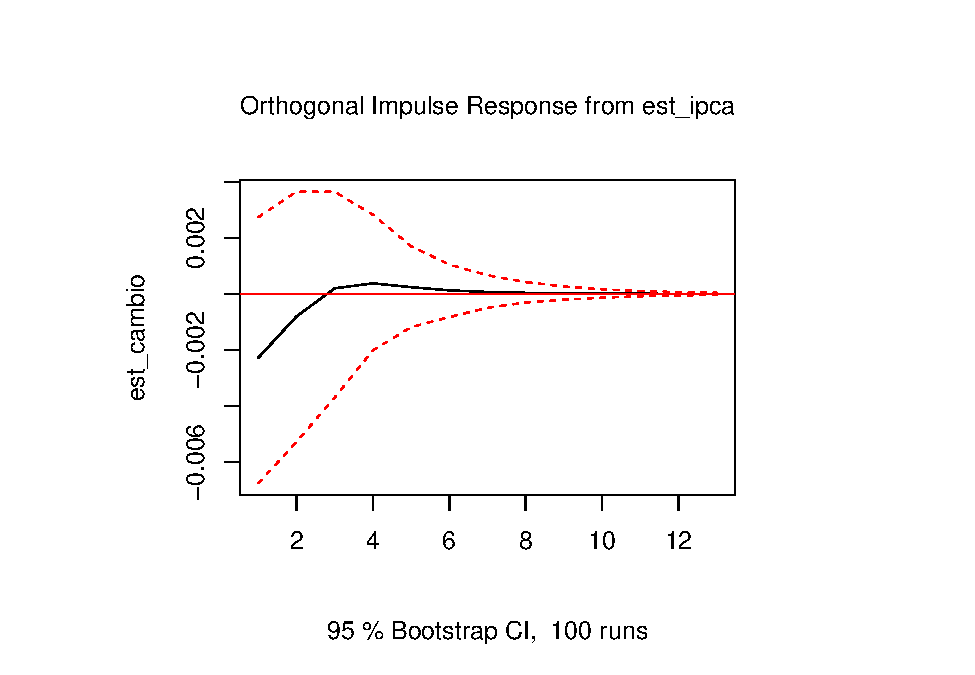
\includegraphics{artigo_files/figure-latex/unnamed-chunk-14-1.pdf}
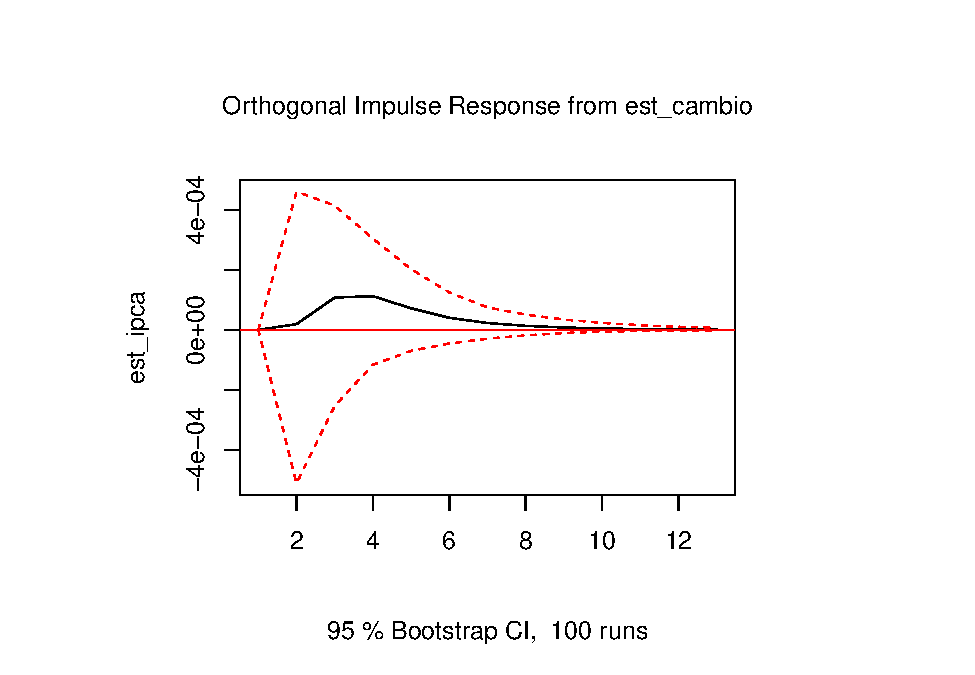
\includegraphics{artigo_files/figure-latex/unnamed-chunk-14-2.pdf}
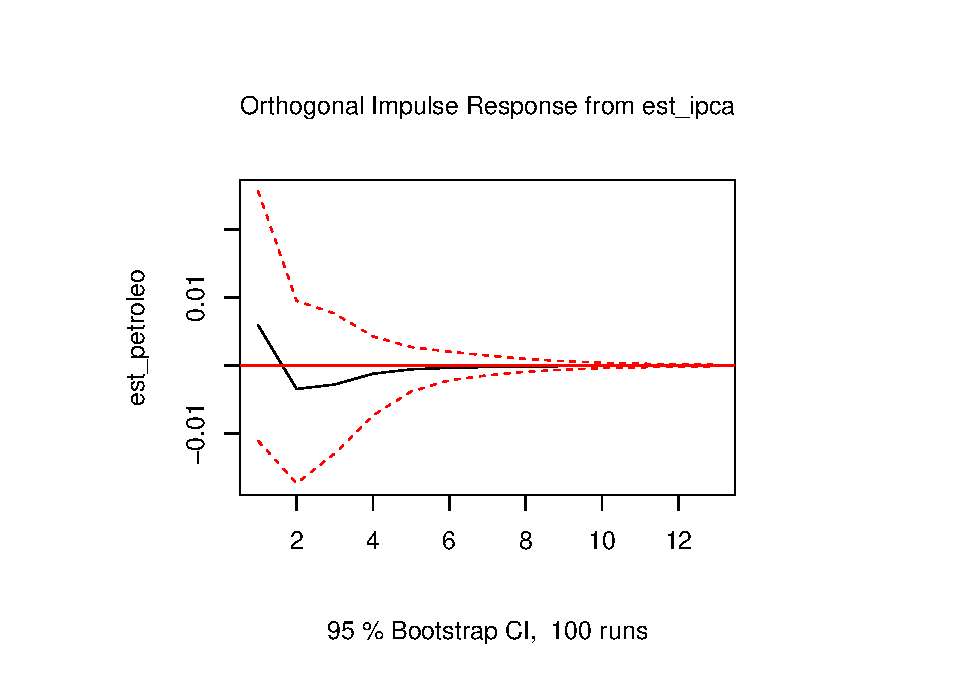
\includegraphics{artigo_files/figure-latex/unnamed-chunk-14-3.pdf}
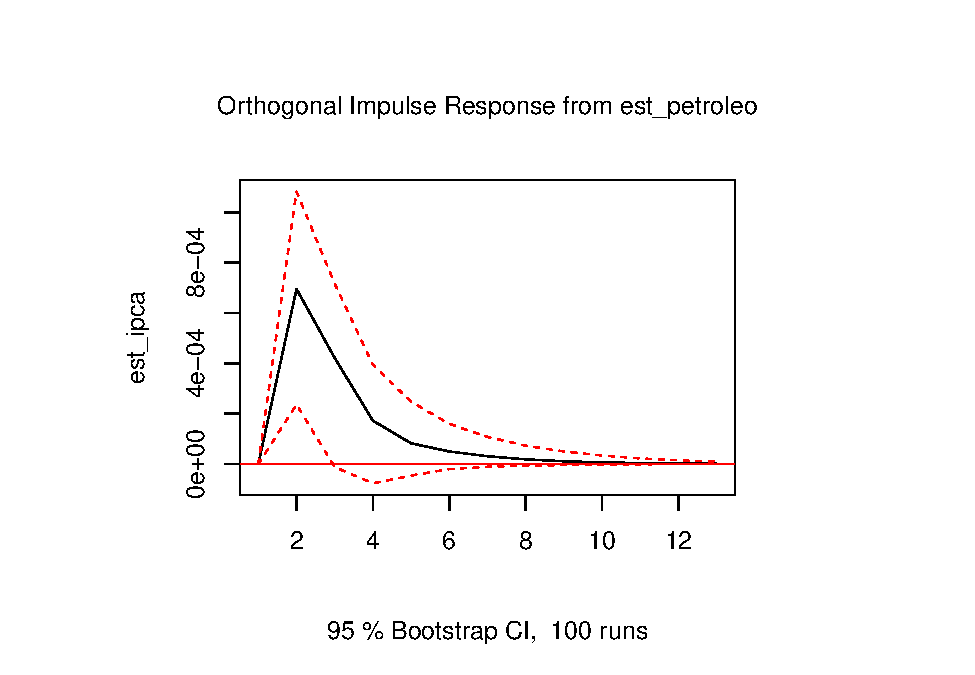
\includegraphics{artigo_files/figure-latex/unnamed-chunk-14-4.pdf}
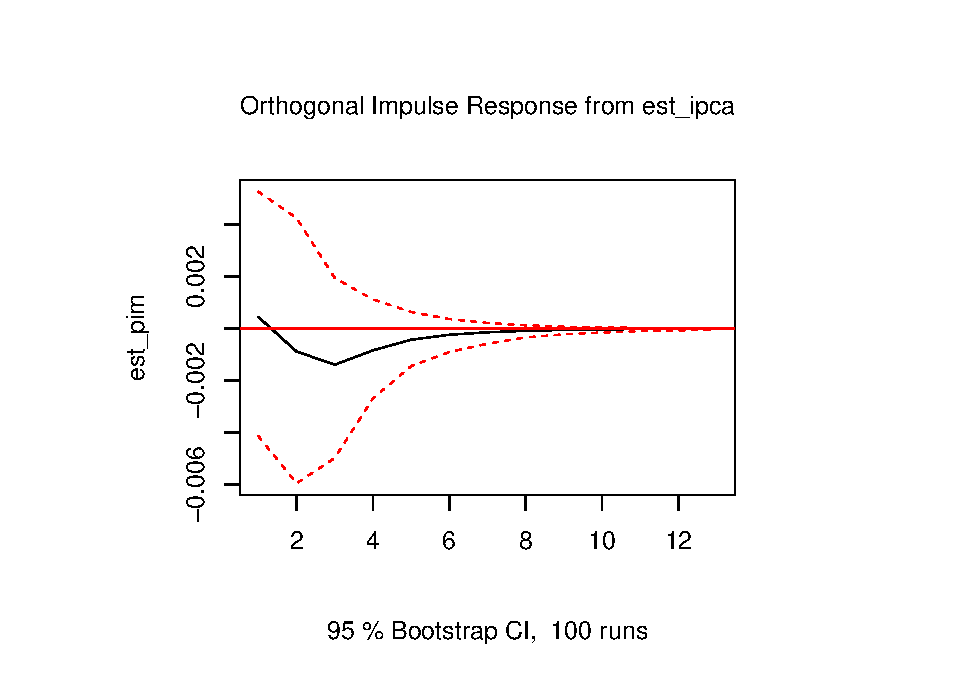
\includegraphics{artigo_files/figure-latex/unnamed-chunk-14-5.pdf}
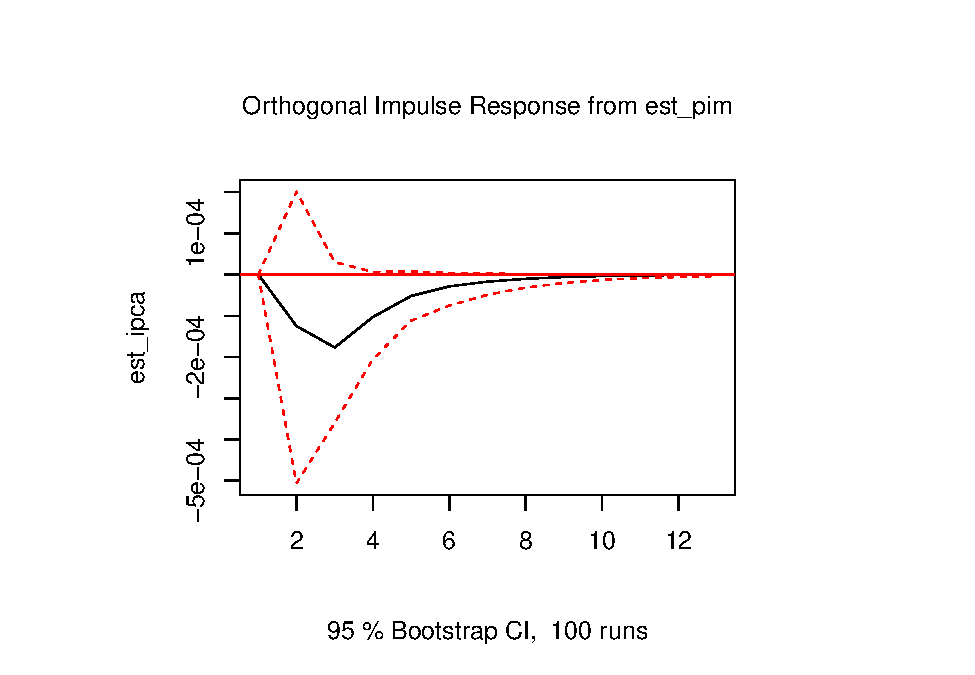
\includegraphics{artigo_files/figure-latex/unnamed-chunk-14-6.pdf}
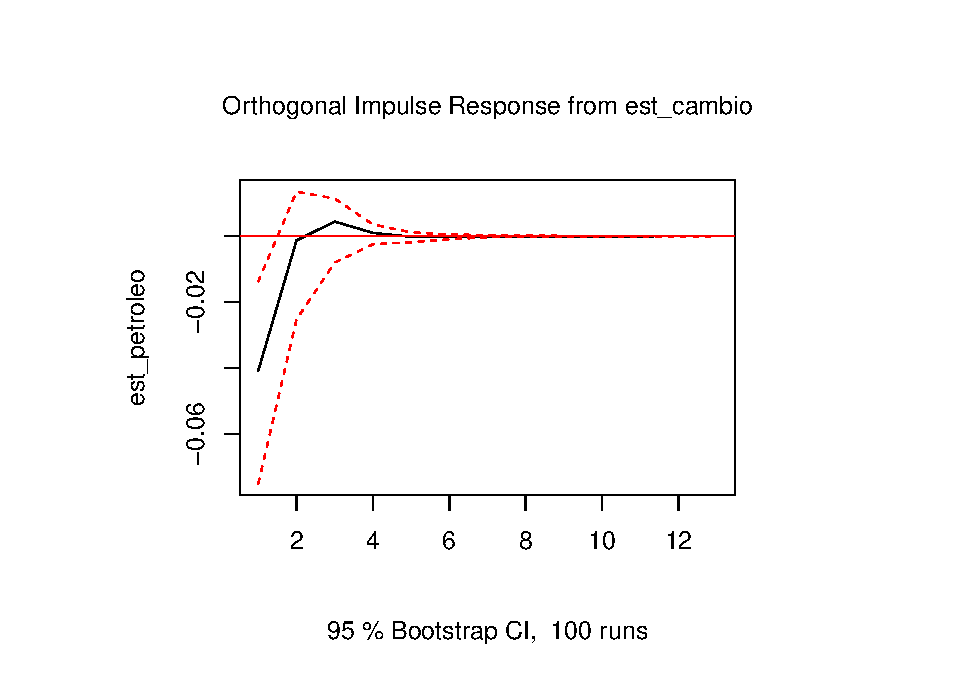
\includegraphics{artigo_files/figure-latex/unnamed-chunk-14-7.pdf}
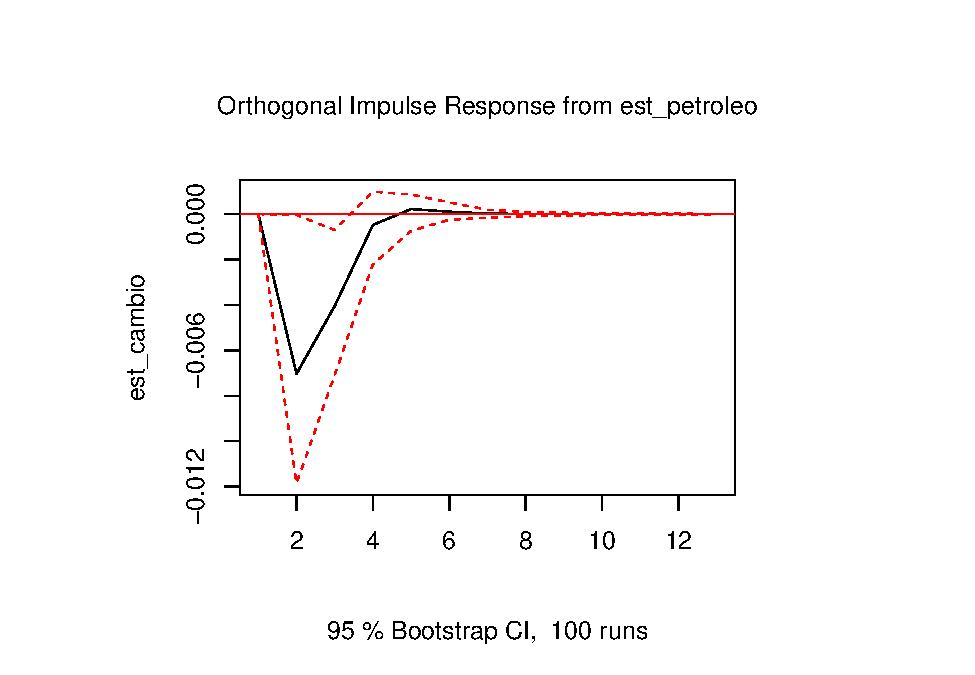
\includegraphics{artigo_files/figure-latex/unnamed-chunk-14-8.pdf}
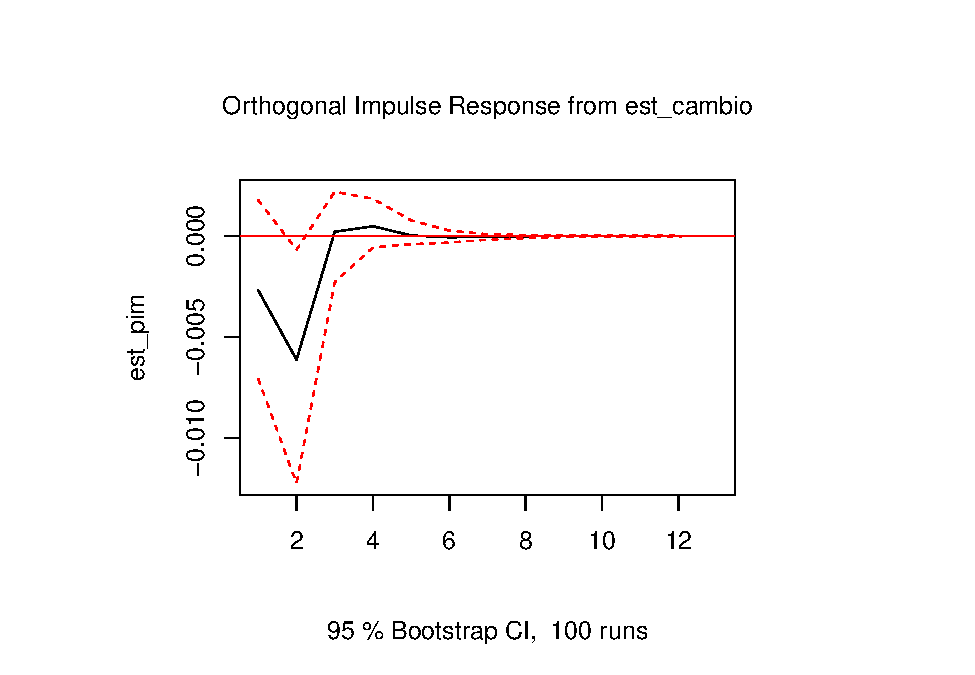
\includegraphics{artigo_files/figure-latex/unnamed-chunk-14-9.pdf}
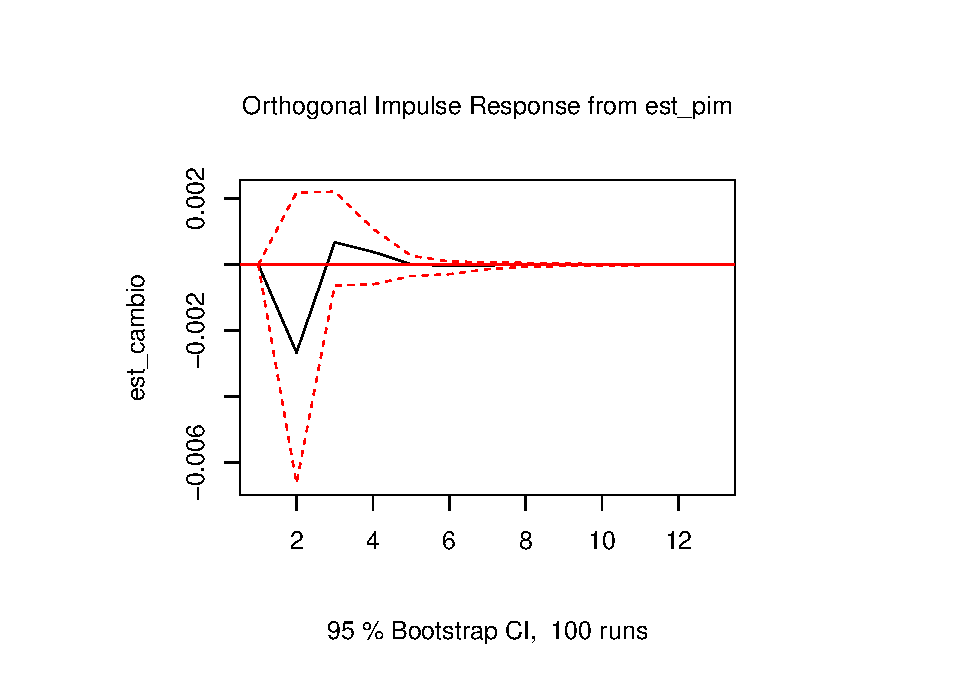
\includegraphics{artigo_files/figure-latex/unnamed-chunk-14-10.pdf}
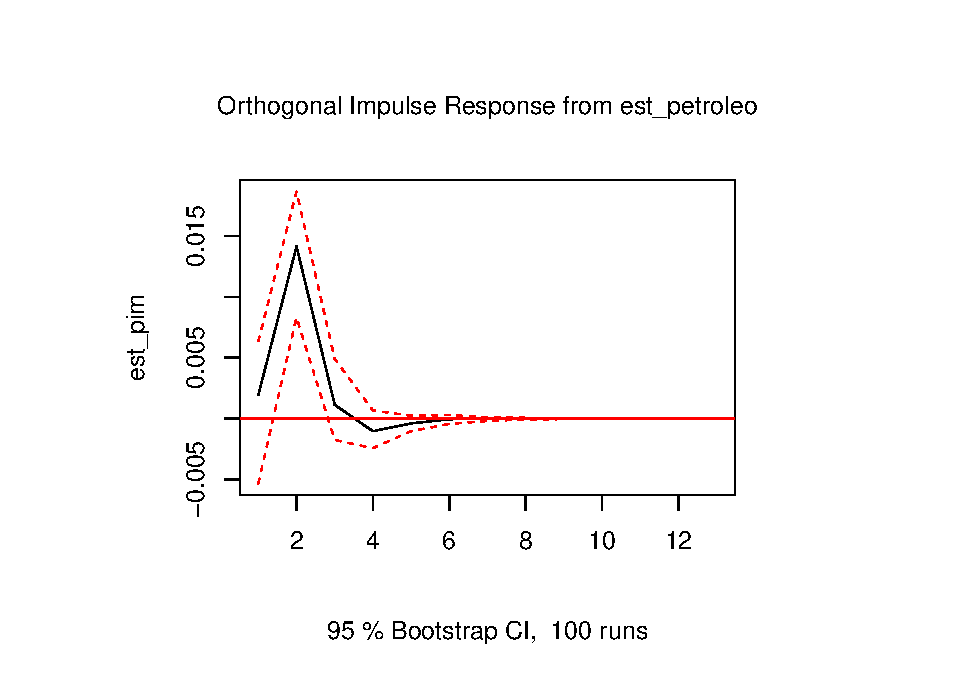
\includegraphics{artigo_files/figure-latex/unnamed-chunk-14-11.pdf}
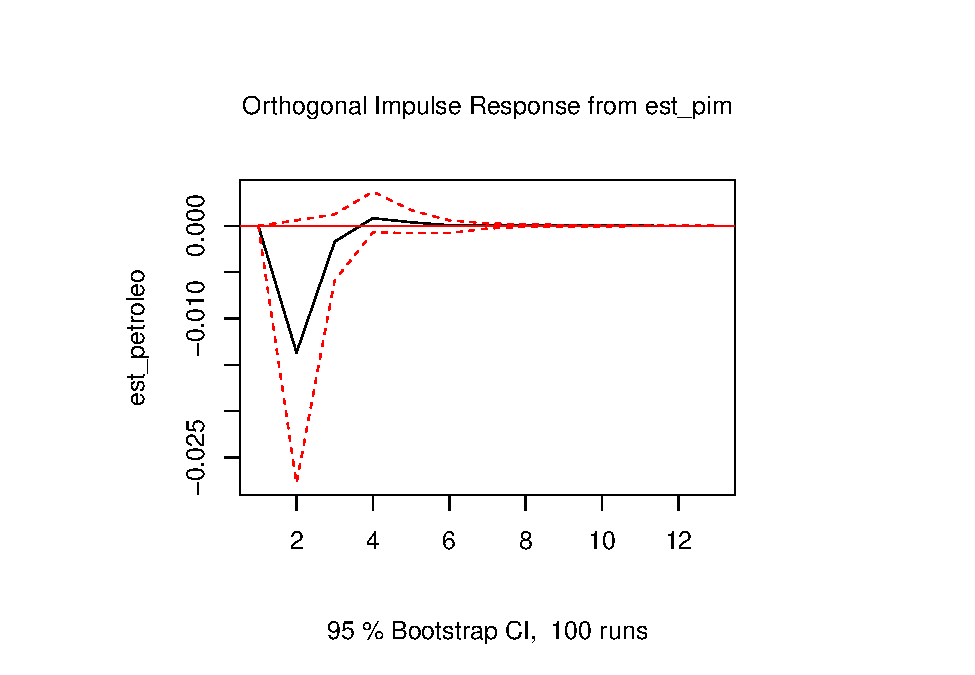
\includegraphics{artigo_files/figure-latex/unnamed-chunk-14-12.pdf}

\bibliographystyle{agsm}
\bibliography{bibliography.bib}


\end{document}
